\documentclass[../masterarbeit.tex]{subfiles}
\begin{document}
	




\subsection{Data}
As mentioned in chapter 3 about machine learning, the acquisition of high quality data is an important and challenging step in the creation of machine learning models, since the quality of the data is directly related to the quality of the models \textcite[]{SUBASI202091}. Especially in the context of predicting avalanche events, the step of collecting homogeneous data and preparing a dataset is a challenge, wich is caused by the fact that avalanche events depend on many different variables. The factors that have a significant influence on avalanche release can be divided into three main categories: terrain, snowpack-related and meteorological data.\autocite[]{Bahram:2019} Data from the three categories were used for this case study, wich does not mean that the used data includes all relevant factors. Proximity to watercourses, for example, can be a terrain-related factor affecting avalanche release \textcite[]{Bahram:2019} and is not included in this study data. The process of preparing the dataset, as well as the origin and composition of the data is explained in this chapter.

\subsubsection{Origin of the data}

The data used for the case study of this paper were provided by the in-house avalanche warning service of the energy company VERBUND AG, headquartered in 1010 Vienna, Austria. Verbund represents Austria's largest and most environmentally friendly  energy company and is one of the largest producer of electricity from hydropower in Europe. It was founded in 1947 with the name Österreichische Elektrizitätswirtschafts-AG. The hydropower plant in Kaprun was one of the first two power plants operated by Verbund AG. \autocite[]{Verbund:2022} The companies strategy slogan "With our power to a green future” \autocite[]{Verbund:2022}, shows the company's intentions to promote environmentally conscious and future-oriented energy production. The company states that it obtains almost 100\% of its electricity from renewable sources and 95\% especially from 129 hydroelectric power plants in Austria and Germany. The electricity is mainly generated from hydro, wind and photovoltaic power plants. In addition, this is supported by gas-fired thermal power plants. The companies goals is to produce completely CO2 free electricity. \autocite[]{Verbund:2022} 
The companies strategy slogan "With our power to a green future” \autocite[]{Verbund:2022}, shows the company's intentions to promote environmentally conscious and future-oriented energy production. 
The company-owned avalanche warning service of the storage power plants in the Hohe Tauern is located in Kaprun, Austria. It was initiated in 1956 due to some heavy avalanches during the construction of the power plants in order to ensure the protection of employees as well as plant and operational safety.
\begin{figure}[h]
    \centering
    \includegraphics[scale=0.17]{Lawinenkartasta.png}
    \source{Avalanche warning service of Verbund AG in Kaprun}
    \caption{The avalanche map of the avalanche warning service of Verbund AG in Kaprun shows the 39 avalanche lines.}
\end{figure} \\
The data were recorded in the vicinity of the Mooserboden storage power plant for 39 avalanche paths. The paths are represented in the avalanche map shown in figure 14. The map was created by the avalanche warning service of Verbund AG in Kaprun. It shows the avalanche prone zones of the study area, to give the avalanche warning service an orientation for their forecasts of the day. The background for the exceptionally accurate recordings of avalanches is the need for the most accurate possible prediction of avalanches in the 39 avalanche lines around the power plant. In the moths from May to Oktober the area is also a touristic spot managed by the Verbund AG\textcite[]{VerbundKaprun:2022}. Accurate forecasting is of great importance to ensure the safety of the employees working in the areas of the avalanche lines. The power plant is part of the Kaprun power plant group, which includes both pumped and storage power plants. The power plant group is operated by Verbund Hydro Power and is located in Salzburg on the edge of the Hohe Tauern at 2040 meters above sea level and is surrounded by the over 3000 meter high mountains of the Glockner group including the Großglockner, wich is the highest mountain in Austria. \autocite[]{VerbundKaprun:2022}
 
 


\subsubsection{Meteorological Data}
Meteorological data are one of the most important factors to initiate snow avalanches \textcite[]{Bahram:2019}. The meteorological data used for this case study were provided by the avalanche warning service in Kaprun in the form of table Mooser\_Wetter\_Daten.
This data table includes meteorological for each day in the months from november to may in the period from 1953 to 2022. Not all columns of the table are complete and some are not filled at all, therefore mainly columns that will be used in the further course of the work are mentioned in the following. The table contains data about the date as well as the winter season, the snow height, the precipitation, the air temperatures at the times 7:00, 14:00 and 19:00 as well as the snow temperature, the wind direction, the wind force, the snow sinking depth, the day weather as well as the weather from the day before, the snow depth, the clouds, the new snow, as well as the avalanche degree. The data from this table has been collected manually and homogoeneous by the team of the avalanche warning service. All of this factors can affect the triggering of snow avalanche events. How relevant the individual features are for the predictions with the three machine learning models used in this study, is described in more detail in the remainder of this thesis.



\subsubsection{Avalanche related data}
The table Allg\_Lawinen\_Abgänge represents general data about all recorded avalanches of the 39 avalanche lines in the area and for the same time period as the meteorological data from the table Mooser\_Wetter\_Data. The snow avalanches have been manually recorded by the avalanche warning service since its initiation in 1956 to get the possibility to analyze the influence of the different factors on the triggering of snow avalanches and to make a good forecast for the day possible. The table contains data such as the time and date when the avalanche was recorded, the type of avalanche, the old ID of the avalanche line where the avalanche went down, the volume of the avalanche, the general weather conditions at the time of the avalanche, the wind direction and speed, the temperature as well as snow height and new snow fallen since the day before, the danger level on the day of the avalanche and a comment of the person who recorded the avalanche event. The meteorological data shown in this table are not used in this study, because the data from the table Mooser\_Wetter\_Daten are homogeneous and available for each day of the winter season, also it would be redundant to use both .
Another table of the database named kaplawstr contains additional information about the avalanche lines. The old and the new code of the avalanche are the only columns from this table used in context of this master thesis. and mainly to connect tables wich each other.

\subsubsection{Topographical Data}
Several of the studies mentioned in chapter 2 on Related work indicate that the influence of topographic factors on the occurrence of avalanche events is a non-negligible one, since these data represent the slopes.\autocite[]{Tiwari:2021} \autocite[]{Bahram:2019} 
The topographical data is recorded in a database table called TOPP. This table contains several rows for each avalanche line, wich can be identified by the new avalanche line code. The table includes for each row the new avalanche line code, the mean slope exposition, the minimum, maximum and mean slope, the altitude of the slope as well as the orientation of the slope. The table also contains various other data columns. These are not used in the further course of the work, since they cannot be assigned to the individual avalanche lines in general, but are connected with individual avalanches, which are not allocated to them in the context of this work. 




\subsubsection{Data Preparation}
 
The database tables Allg\_Lawinen\_Abgänge (Avalanche related data), kaplawstr (contains the old as well as the new avalanche line IDs), TOPP (Topographical Data) and Mooser\_Wetter\_Daten (Meteorological data) wich are already described in the previous chapters were merged into a homogeneous data set in the context of this master thesis. This section describes the data preparation process including the merging of the data tables to a homogeneous set and the removal of redundant and not adequately filled data columns. \\
The tables include data from 1944 to 2022. The recording of the avalanches in the past was not completely homogenous and incomplete. Table one shows a total listing of the sum of avalanches recored per winter season winter for each winter season included in the dataset. This can be shown above all by the fact that in the seasons from 1944 to the season of 1988/1989 in average, there are 22.0769 snow avalanches per season recorded. In comparison, in the seasons from 1989/1990 to season 2021/2022 the average of recorded snow avalanches is 81.636. The table gives an understanding about how less avalanches are recorded per season before the season of 1989/1990 in comparison to the seasons since 1989/1990. With the exception of a few outliers, hardly any avalanches were recorded in these years, and in the cases of the seasons 1971/ 1972, 1976/ 1977 and 1983/ 1984 there were no avalanches recorded at all. In order to increase the homogeneity of the data and decrease the bias caused through the unbalanced ratio between avalanche and non-avalanche samples, wich Chawla, M. and Singh, A. mentioned in their study about an data efficient approach of snow avalanche forecasting \textcite[]{nhess-2021-106}, all data outside the period from season 1989/1990 to season 2021/2022 were removed from the database tables.
Subsequently to this measure the kaplawstr table has been merged to the Allg\_Lawinen\_Catalog table using the old avalanche line ID. This adds the associated new avalanche code and avalanche name to each avalanche, which are used as additional ID. The connection is necessary because the TOPP table, which represents the topographic data for the avalanche routes, does not contain the old avalanche line ID. In the course of this step, all lines that were labeled with the avalanche line name "all avalanches" also have been removed. These are not included in the kaplawstr table, since this does not represent an exact departure of an avalanche in one of the avalanche lines, but only states that in many of the avalanche lines small avalanches have departed. \\


\begin{table}
    \centering
    \begin{tabular}{|l|l|}
    \hline
        Intervall & Avalanche \\ \hline
        1956/ 1957 & 11 \\ \hline
        1957/ 1958 & 4 \\ \hline
        1958/ 1959 & 7 \\ \hline
        1959/ 1960 & 62 \\ \hline
        1964/ 1965 & 8 \\ \hline
        1965/ 1966 & 8 \\ \hline
        1966/ 1967 & 15 \\ \hline
        1967/ 1968 & 9 \\ \hline
        1968/ 1969 & 3 \\ \hline
        1969/ 1970 & 20 \\ \hline
        1970/ 1971 & 22 \\ \hline
        1971/ 1972 & 0 \\ \hline
        1972/ 1973 & 67 \\ \hline
        1973/ 1974 & 31 \\ \hline
        1974/ 1975 & 78 \\ \hline
        1976/ 1977 & 0 \\ \hline
        1979/ 1980 & 27 \\ \hline
        1980/ 1981 & 40 \\ \hline
        1981/ 1982 & 29 \\ \hline
        1982/ 1983 & 27 \\ \hline
        1983/ 1984 & 0 \\ \hline
        1984/ 1985 & 10 \\ \hline
        1985/ 1986 & 24 \\ \hline
        1986/ 1987 & 37 \\ \hline
        1987/ 1988 & 17 \\ \hline
        1988/ 1989 & 18 \\ \hline
        1989/ 1990 & 66 \\ \hline
        1990/ 1991 & 55 \\ \hline
        1991/ 1992 & 133 \\ \hline
        \end{tabular}
        \begin{tabular}{|l|l|}
        \hline
        Intervall & Avalanche \\ \hline
        1992/ 1993 & 80 \\ \hline
        1993/ 1994 & 47 \\ \hline
        1994/ 1995 & 93 \\ \hline
        1995/ 1996 & 3 \\ \hline
        1996/ 1997 & 19 \\ \hline
        1997/ 1998 & 18 \\ \hline
        1998/ 1999 & 90 \\ \hline
        1999/ 2000 & 128 \\ \hline
        2000/ 2001 & 89 \\ \hline
        2001/ 2002 & 124 \\ \hline
        2002/ 2003 & 84 \\ \hline
        2003/ 2004 & 92 \\ \hline
        2004/ 2005 & 97 \\ \hline
        2005/ 2006 & 100 \\ \hline
        2006/ 2007 & 40 \\ \hline
        2007/ 2008 & 86 \\ \hline
        2008/ 2009 & 79 \\ \hline
        2009/ 2010 & 52 \\ \hline
        2010/ 2011 & 52 \\ \hline
        2011/ 2012 & 150 \\ \hline
        2012/ 2013 & 121 \\ \hline
        2013/ 2014 & 55 \\ \hline
        2014/ 2015 & 75 \\ \hline
        2015/ 2016 & 66 \\ \hline
        2016/ 2017 & 67 \\ \hline
        2017/ 2018 & 133 \\ \hline
        2018/ 2019 & 177 \\ \hline
        2019/ 2020 & 67 \\ \hline
        2020/ 2021 & 130 \\ \hline
        2021/ 2022 & 26 \\ \hline
    \end{tabular}
    \caption{recorded Avalanches per Season}
\end{table}



\begin{lstlisting}[language=Python, caption=calculation of TOPP data for every avalanche line]
TOPP = kaplawstr['Code_neu'].apply(lambda x: TOPP.loc[TOPP['Lawinencode'] == x].mean())
\end{lstlisting} 
In the second step, the average values for all columns from the associated avalanches were calculated from the TOPP table for each avalanche line to get representative values for these columns. This is important, because the recorded avalanches from the Allg\_Lawinen\_Abgänge table can not be directly assigned to the TOPP rows but to the avalanche lines. The python code shown in Listing 1 demonstrates this process. \\
By this measure, one row is created for each avalanche line. The table contained without this procedure a total of 1905 rows. In the default state, the table could not have been connected to the other data tables. Another way to get only one row per avalanche stroke would be to select a random value for the respective stroke. The reason for taking the average value is that there are not the same number of lines for all avalanche lines and the values of the individual lines per avalanche line do not differ greatly from each other. Thus, the average value represents the entirety of the lines per stroke consistently. The topographic data from the newly assembled TOPP table was then merged to the recorded avalanches in the entire dataset using the new avalanche ID. \\~\\
Subsequently, these avalanches were assigned to the daily recorded meteorological data of the Mooser\_Wetter\_Data table by an outer join, so as result there is at least one row per day in the dataset. In cases where several large avalanches have occurred at the same day, the dataset contains one row per avalanche and each Includes the meteorological data for this day plus the topographical data for the avalanche line. \\~\\
In order to train a machine learning algorithm with the aim of predicting snow avalanches for topographically defined slopes in conjunction with the meteorological data available for this study, the topographical data must also be mapped onto the days without avalanches. The algorithm needs this information, as the data set would otherwise only contain topographic data directly related to avalanches. This would mean that the machine learning algorithm learns that as soon as the topographical data of a slope is available also an avalanche is triggered.
\\
\begin{lstlisting}[language=Python, caption=mapping random sample lines of topographical data onto the rows of non avalanche days]
for i in gesamt_df.index:
    if(pd.isnull(gesamt_df['meanExpo'][i])):
        sample = TOPP.sample(1)
        gesamt_df['meanExpo'][i] = sample['meanExpo'].values[0]
        gesamt_df['meanSlope'][i] = sample['meanSlope'].values[0]
        gesamt_df['stdDevSlope'][i] = sample['stdDevSlope'].values[0]
        gesamt_df['MinSlope'][i] = sample['MinSlope'].values[0]
        gesamt_df['MaxSlope'][i] = sample['MaxSlope'].values[0]
        gesamt_df['Altitude'][i] = sample['Altitude'].values[0]
\end{lstlisting} 
The consequence of this is that the topographic data must also be mapped to the days without avalanches. Because these days are not connected to an avalanche line ID and an even distribution on the slopes on these days is required, random avalanche lines were picked from the calculated mean values of the TOPP table and mapped onto the non-avalanche days. Listing 2 shows how the avalanche line is randomly picked out of the modified TOPP table and the six columns of the picked row wich define the avalanche line topographical are mapped on the days without topographical information. This is shown in form of the corresponding Python code.\\ 
The resulting dataset maps 7021 rows and 139 columns. 2728 of these rows are recorded avalanches departures. This results in a data set consisting of 38.7\% avalanche samples and 61.3\% non-avalanche samples. The number of non-avalanche samples is therefore larger than the number of avalanche samples. Because of this, a bias can occur due to the greater number of non-avalanches. The evaluation of the three machine learning models will indicate whether such a bias is present. The dataset contains columns that are redundant, empty, sparsely filled or contain information wich can not be used to train a machine learning algorithm. Figure 15 shows a heatmap of the Nan values in the dataset, to get an overview about how many columns are sparse or incomplete. All white marked parts of the heatmap stand for Nan values in the dataset.  As mentioned in chapter 3.1 about feature selection, these columns can cause a huge cost in computation time, decrease the prediction performance and increase the error rate. This requires the measure to remove all columns with these characteristics or fill their values.
\\
\begin{figure}[h]
    \centering
    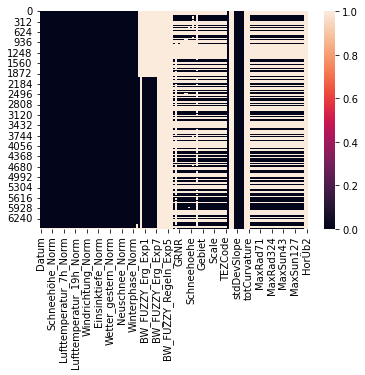
\includegraphics[scale=1.0]{heatmap_nanValues.png}
    \source{created by the author}
    \caption{Heatmap to show the distribution of Nan values in the dataset}
\end{figure}
\\
In addition, a new column was added to the dataset, which contains either a 1 in case of an avalanche or a 0 in case no avalanche has occurred. This column is added to make it possible to predict  whether an avalanche will occur or not. To train a machine learning algorithm on predicting whether an avalanche will go down from a topographical specified slope, wich is the specific aim of this master thesis, all features that can be used to directly and without any other features determine whether an avalanche will descend must be removed from the dataset.\\
The columns, wich are dropped for that reason are: \\
'Datum','Intervall','ZEIT','Lawinenabgänge', 'ID', 'Volumen', 'Lawinen\_Art'
After dropping this features the dataset includes 41 features. These columns include 25 meteorological factors, nine snowpack related features and six topographical factors and the column avalanche column wich says if this sample is an avalanche or a non-avalanche one.In the further course of the work the names of the data columns are used. For this reason and to get an overview about the dataset, table two shows all the features contained in the dataset in conjunction with their associated description. 




\begin{table}
    \centering
    \begin{tabular}{|l|l|}
    \hline
        Column Name & Description \\ \hline
        Datum & The samples date \\ \hline
        Intervall & The winter season in wich the sample was recorded \\ \hline
        Schneehöhe & The snow height \\ \hline
        Schneehöhe\_Norm & The normalized snow height \\ \hline
        Niederschlag & The rainfall \\ \hline
        Lufttemperatur\_7h & The air temperature at 7am \\ \hline
        Lufttemperatur\_7h\_Norm & The normalized air temperature at 7am \\ \hline
        Lufttemperatur\_7h\_Gew & The weighted air temperature at 7am \\ \hline
        Lufttemperatur\_14h & The air temperature at 2pm \\ \hline
        Lufttemperatur\_14h\_Norm & The normalized air temperature at 2pm \\ \hline
        Lufttemperatur\_14h\_Gew & The weighted air temperature at 2pm \\ \hline
        Lufttemperatur\_19h & The air temperature at 7pm \\ \hline
        Lufttemperatur\_19h\_Norm & The normalized air temperature at 7pm \\ \hline
        Lufttemperatur\_19h\_Gew & The weighted air temperature at 7pm \\ \hline
        Schneetemperatur & The snow temperature \\ \hline
        Schneetemperatur\_Norm & The normalized snow temperature \\ \hline
        Schneetemperatur\_Gew & The weighted snow temperature \\ \hline
        Windrichtung & The wind direction \\ \hline
        Windrichtung\_Norm & The normalized wind direction \\ \hline
        Windrichtung\_Gew & The weighted wind direction \\ \hline
        Windstärke & The wind speed \\ \hline
        Windstärke\_Norm & The normalized wind speed \\ \hline
        Windstärke\_Gew & The weighted wind speed \\ \hline
        Einsinktiefe & the snow sinking depth \\ \hline
        Einsinktiefe\_Norm & the normalized snow sinking depth \\ \hline
        Einsinktiefe\_Gew & The weight snow sinking depth \\ \hline
        Wetter\_akt & The encoded weather of the samples current day \\ \hline
        Wetter\_gestern & The encoded weather of the day before \\ \hline
        Wolken & The encoded number of clouds \\ \hline
        Wolken\_Norm & The normalized encoded number of clouds \\ \hline
        Neuschnee\_x & The new snow on the samples current day \\ \hline
        Neuschnee\_Norm & The normalized new snow on the samples current day \\ \hline
        Neuschnee\_Gew & The weighted new snow on the samples current day \\ \hline
        ID & The new avalanche ID \\ \hline
        meanExpo & The mean slope exposition \\ \hline
        meanSlope & The mean slope \\ \hline
        stdDevSlope & The standard deviation of the slop \\ \hline
        MinSlope & The minimum slope \\ \hline
        MaxSlope & The maximum slope \\ \hline
        Altitude & The elevation above sea level \\ \hline
        Avalanche & The binary value if the sample is an avalanche or a non avalanche one \\ \hline
    \end{tabular}
    \caption{The columns of the resulting dataset, in combination with their descriptions}
\end{table}







\end{document}